\documentclass[aspectratio=169]{beamer}

\usepackage{amsmath}
\usepackage{amssymb}
\usepackage{array}
\usepackage{xcolor}
\usepackage{tikz}

\usetikzlibrary{shapes.geometric}
\usetikzlibrary{arrows}
\usetikzlibrary{calc,decorations.markings,math,arrows.meta}

\newcommand{\com}{\mathsf{Com}}

\definecolor{monerodark}{HTML}{4D4D4D}
\definecolor{monerorange}{HTML}{F26822}
\definecolor{text}{RGB}{248, 248, 242}

\setbeamercolor{normal text}{fg=text, bg=monerodark}
\setbeamercolor{title}{fg=text, bg=monerorange!90}
\setbeamercolor*{titlelike}{use=normal text}
\setbeamercolor*{frametitle}{use=normal text, bg=monerodark!80}
\setbeamercolor*{item}{fg=monerorange}

\setbeamertemplate{footline}[frame number]
\beamertemplatenavigationsymbolsempty

\title{How Do We Design Secure Protocols?}
\author{Aaron Feickert, Ph.D.}
\date{Monero Konferenco \\ 7 June 2024}

\begin{document}

\frame{\titlepage}

\begin{frame}{Acknowledgments and disclaimer}
	The author is head of research at \textbf{Cypher Stack}. \\~\\

	The material in this presentation is for informational use only, has not undergone formal external review, and does not constitute professional advice of any kind.
\end{frame}

\begin{frame}
    When we look at a cryptographic design and discuss \textbf{security}, what does that mean?

    \vspace{30px}

    \begin{center}
        \includegraphics[width=50px]{images/lock.png}
    \end{center}
\end{frame}

\begin{frame}{Our approach}
    There are different ways to formalize and prove that a cryptographic design is secure. \\~\\

    We'll show some strategies that are often used to examine the security of cryptographic systems. \\~\\

    In particular, we'll show this using some relevant examples. \\~\\

    This is \textbf{not} a deep dive, or comprehensive!
\end{frame}

\begin{frame}{Example: signatures}
    \begin{tabular}{>{\arraybackslash}m{40px} >{\arraybackslash}m{320px}}
        \includegraphics[width=30px]{images/pen.png} & \textbf{Signatures} are used for certain types of authentication. \\~\\
    \end{tabular}

    \begin{tabular}{>{\arraybackslash}m{40px} >{\arraybackslash}m{320px}}
        \includegraphics[width=30px]{images/key.png} & Given a signing key and message, a signer produces a signature. Given a verifying key, a verifier checks the signature. \\~\\
    \end{tabular}

    Cryptographically, we break this up into formalized \textbf{algorithms}:
    \begin{itemize}
        \item \textbf{Key generation}: Produce a signing and verifying key.
        \item \textbf{Sign}: Take a signing key and message, and produce a signature.
        \item \textbf{Verify}: Take a verifying key, message, and signature; and check validity.
    \end{itemize}
\end{frame}

\begin{frame}{Security model}
    \begin{tabular}{>{\arraybackslash}m{40px} >{\arraybackslash}m{320px}}
        \includegraphics[width=30px]{images/die.png} & We formalize the \textbf{security model} using \textbf{games} played by an \textbf{adversary}. \\~\\
    \end{tabular}

    Each property in the security model has a game we must define.
    If the adversary can win the game, it has broken the property. \\~\\

    We'll use a \textbf{security proof} to show that no adversary can win the game, so the property holds.
\end{frame}

\begin{frame}{Unforgeability}
    \begin{tabular}{>{\arraybackslash}m{40px} >{\arraybackslash}m{320px}}
        \includegraphics[width=30px]{images/pen.png} & We don't want signatures to be forged without the signing key, so we'll define a \textbf{forgery} game. \\~\\
    \end{tabular}

    The adversary's goal is to give us a valid signature on a message when it doesn't know the signing key. \\~\\

    If the adversary can't win this game, the signature design is \textbf{unforgeable}.
\end{frame}

\begin{frame}{The game}
    \begin{figure}
        \begin{tikzpicture}[thick]
            % Header
            \node [rectangle,draw] (us) {Us};
            \node [rectangle,draw,right=200px,at=(us)] (adversary) {Adversary};

            % Step 1: keys
            \node [below=10px,at=(us.south)] (step1_us_key) {\includegraphics[width=20px]{images/oldkey.png} \includegraphics[width=20px]{images/key.png}};
            \node [below=10px,at=(adversary.south)] (step1_adv_key) {\includegraphics[width=20px]{images/key.png}};

            % Step 2a: message
            \node [below=5px,at=(step1_adv_key.south)] (step2_adv_message) {\includegraphics[width=20px]{images/page.png}};
            \node [below=5px,at=(step1_us_key.south)] (step2_us_message) {\includegraphics[width=20px]{images/page.png}};
            
            % Step 2b: signature
            \node [below=5px,at=(step2_us_message.south)] (step2_us_sign) {\includegraphics[width=20px]{images/pen.png}};
            \node [below=5px,at=(step2_adv_message.south)] (step2_adv_sign) {\includegraphics[width=20px]{images/pen.png}};

            % Step 3: repeat
            \node [below=5px,at=(step2_us_sign.south)] (step3_us_dots) {$\vdots$};
            \node [below=5px,at=(step2_adv_sign.south)] (step3_adv_dots) {$\vdots$};

            % Step 4: message and signature
            \node [below=5px,at=(step3_adv_dots.south)] (step4_adv_sign) {\includegraphics[width=20px]{images/page.png} \includegraphics[width=20px]{images/pen.png}};
            \node [below=5px,at=(step3_us_dots.south)] (step4_us_sign) {\includegraphics[width=20px]{images/page.png} \includegraphics[width=20px]{images/pen.png}};

            \draw [-{Latex[scale=1.5]}] (step1_us_key) -- (step1_adv_key) node[anchor=south,midway] {send verification key};
            \draw [-{Latex[scale=1.5]}] (step2_adv_message) -- (step2_us_message) node[anchor=south,midway] {receive message};
            \draw [-{Latex[scale=1.5]}] (step2_us_sign) -- (step2_adv_sign) node[anchor=south,midway] {send signature};
            \draw [-{Latex[scale=1.5]}] (step4_adv_sign) -- (step4_us_sign) node[anchor=south,midway] {receive signed message};
        \end{tikzpicture}
    \end{figure}
\end{frame}

\begin{frame}{Adversary powers}
    \begin{tabular}{>{\arraybackslash}m{40px} >{\arraybackslash}m{320px}}
        \includegraphics[width=30px]{images/muscle.png} & Notice that we gave the adversary some powers. \\~\\
    \end{tabular}
    
    \begin{itemize}
        \item It received the verifying key.
        \item It could ask us to sign any messages it chose. \\~\\
    \end{itemize}

    \begin{tabular}{>{\arraybackslash}m{40px} >{\arraybackslash}m{320px}}
        \includegraphics[width=30px]{images/globe.png} & The powers given to an adversary in a game should reflect the real world as much as possible.
    \end{tabular}
\end{frame}

\begin{frame}{Security proof}
    The unforgeability property is general; it can apply to many different signature designs:
    \begin{itemize}
        \item ECDSA
        \item Schnorr
        \item RSA
        \item ... \\~\\
    \end{itemize}

    A security proof is specific to a given design. \\~\\

    \begin{tabular}{>{\arraybackslash}m{40px} >{\arraybackslash}m{320px}}
        \includegraphics[width=30px]{images/collision.png} & We'll show that if an adversary could win the game, it could solve a problem believed to be hard.
    \end{tabular}
\end{frame}

\begin{frame}{Tricking the adversary}
    \begin{tabular}{>{\arraybackslash}m{40px} >{\arraybackslash}m{320px}}
        \includegraphics[width=30px]{images/collision.png} & Basically, we want to trick the adversary into solving a hard problem for us by winning our game. \\~\\
    \end{tabular}

    For Schnorr signatures, the hard problem is the \textbf{discrete logarithm problem}, which has its own game! \\~\\

    The unforgeability proof shows that we can win the discrete logarithm game by passing information along to and from the forgery game adversary. \\~\\

    \begin{tabular}{>{\arraybackslash}m{40px} >{\arraybackslash}m{320px}}
        \includegraphics[width=30px]{images/shrug.png} & We don't know for sure that the discrete logarithm game can't be won; we assume it's hard from decades of research and experience.
    \end{tabular}
\end{frame}

\begin{frame}{Example: CLSAG}
    \begin{tabular}{>{\arraybackslash}m{40px} >{\arraybackslash}m{320px}}
        \includegraphics[width=30px]{images/monero.png} & Monero uses a variation of a signature (a \textbf{linkable ring signature}) called CLSAG to authorize transactions. \\~\\
    \end{tabular}

    It has an unforgeability property whose game requires the adversary to produce a signature containing a list of possible verifying keys. \\~\\

    \begin{tabular}{>{\arraybackslash}m{40px} >{\arraybackslash}m{320px}}
        \includegraphics[width=30px]{images/fingers.png} & The game required that the adversary's list of keys be ``honest'' in how they were produced; but this isn't what happens in the real world! \\~\\
    \end{tabular}

    Auditors recommended the game be changed to let the adversary put whatever it wants into the list, giving the adversary more power.
\end{frame}

\begin{frame}{Example: range proofs}
    \begin{tabular}{>{\arraybackslash}m{40px} >{\arraybackslash}m{320px}}
        \includegraphics[width=30px]{images/balance.png} & Part of showing that transactions balance requires a \textbf{range proof}, which asserts that outputs represent a valid (hidden) amount. \\~\\
    \end{tabular}

    In Monero, amounts are represented by taking the value and a mask, and producing a random-looking blob called a \textbf{commitment}.

    \begin{figure}
        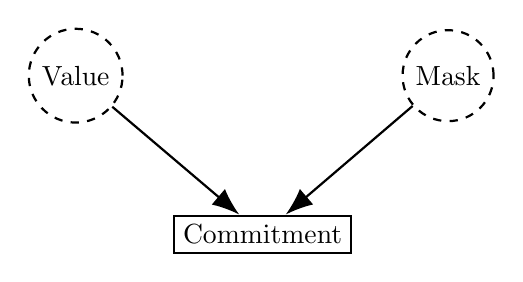
\begin{tikzpicture}[thick]
            \node [rectangle,draw] (commitment) {Commitment};
            \node [circle,draw,dashed,above=50px,left=50px,at=(commitment.north)] (value) {Value};
            \node [circle,draw,dashed,above=50px,right=50px,at=(commitment.north)] (mask) {Mask};

            \draw [-{Latex[scale=1.5]}] (value) -- (commitment);
            \draw [-{Latex[scale=1.5]}] (mask) -- (commitment);
        \end{tikzpicture}
    \end{figure}
\end{frame}

\begin{frame}{Proving relation}
    We want to represent the range proof using a formal \textbf{proving relation} that specifies how public and secret data relate to each other. \\~\\

    \begin{tabular}{>{\arraybackslash}m{40px} >{\arraybackslash}m{100px} >{\arraybackslash}m{220px}}
        \includegraphics[width=30px]{images/unlock.png} & \textbf{Public data} & Commitment \\
        \includegraphics[width=30px]{images/lock.png} & \textbf{Secret data} & Value, mask \\~\\
    \end{tabular}

    The relationship is:
    \begin{itemize}
        \item The commitment was produced from the value and mask.
        \item The value is within a specific range.
    \end{itemize}
\end{frame}

\begin{frame}{Security properties}
    The \textbf{prover} uses the secret data to build a proof. \\~\\

    The \textbf{verifier} uses the public data to verify the proof. \\~\\

    The (informal) security properties for something like a range proof are:
    \begin{itemize}
        \item \textbf{Completeness}: If the prover knows the secret data, the verifier will judge the proof as valid.
        \item \textbf{Soundness}: If the prover doesn't know the secret data, the verifier will judge the proof as invalid.
        \item \textbf{Zero knowledge}: The verifier doesn't learn anything about the secret data.
    \end{itemize}
\end{frame}

\begin{frame}{Soundness}
    A common way to show soundness (the prover knows the secret data) is to build something called an \textbf{extractor}. \\~\\

    The extractor is an algorithm that pretends to be the verifier, and asks the prover to generate multiple proofs for the same public data in a specific technical way. \\~\\

    The extractor shows that it can ``pull out'' the secret data, which shows that the prover knew it to begin with.

    \begin{figure}
        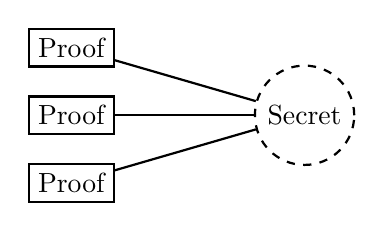
\begin{tikzpicture}[thick]
            \node [rectangle,draw] (p1) {Proof};
            \node [rectangle,draw,below=10px,at=(p1.south)] (p2) {Proof};
            \node [rectangle,draw,below=10px,at=(p2.south)] (p3) {Proof};
            \node [circle,dashed,draw,right=50px,at=(p2.east)] (secret) {Secret};

            \draw [-] (p1) -- (secret);
            \draw [-] (p2) -- (secret);
            \draw [-] (p3) -- (secret);
        \end{tikzpicture}
    \end{figure}
\end{frame}

\begin{frame}{Security properties}
    Monero has used three different range proof designs:
    \begin{itemize}
        \item Borromean ring signatures
        \item Bulletproofs
        \item Bulletproofs+ \\~\\
    \end{itemize}

    Each of these has a different security proof to show the security properties. \\~\\

    \begin{tabular}{>{\arraybackslash}m{40px} >{\arraybackslash}m{320px}}
        \includegraphics[width=30px]{images/globe.png} & These security properties apply very generally, not just to range proofs.
        All we need is a proving relation.
    \end{tabular}
\end{frame}

\begin{frame}{Why these properties?}
    Why is it helpful to have these security properties common to any design that supports a proving relation? \\~\\

    \begin{tabular}{>{\arraybackslash}m{40px} >{\arraybackslash}m{320px}}
        \includegraphics[width=30px]{images/pancakes.png} & The security proofs can stack to build more complex systems! \\~\\
    \end{tabular}

    A complex cryptographic protocol might use something like a range proof as a building block, making the whole construction more modular. \\~\\

    (You can even use this idea for things like Schnorr signatures!)
\end{frame}

\begin{frame}{But wait, there's more!}
    \begin{tabular}{>{\arraybackslash}m{40px} >{\arraybackslash}m{320px}}
        \includegraphics[width=30px]{images/sparkles.png} & There's a whole universe of techniques and approaches to proving security for different cryptographic systems. \\~\\
    \end{tabular}

    Here are some takeaways:
    \begin{itemize}
        \item A security proof is only as good as the underlying security model. If the model doesn't match the real world, the proof may be valid but not useful.
        \item Some common and general security properties are useful because they help layer simpler systems into more complex ones.
        \item Formal security is tricky but essential for building robust systems.
    \end{itemize}
\end{frame}

\begin{frame}{Questions?}
	\Large
	\begin{center}
		\begin{tabular}{ll}
			\textbf{Slides} & \url{github.com/AaronFeickert/monkon2024} \\
			\\
			\textbf{Email} & \texttt{aaron@cypherstack.com}
		\end{tabular}
	\end{center}
\end{frame}

\end{document}
